\begin{frame}{}
    \begin{center}
        \LARGE Motivaci\'on y Marco Teorico
    \end{center}
\end{frame}


\begin{frame}{Motivaci\'on}

\begin{itemize}
    \item Estudio por medio de simulaci\'on de un modelo teorico que predice la creaci\'on de nuevas particulas y fuerzas fundamentales 
    \item Dichas particulas conocidas como fotones oscuros (Dark photons) son uno de los candidatos para explicar la composici\'on de la materia oscura en el universo 
    
\end{itemize}

\end{frame}

\begin{frame}{Objetivos}

\begin{itemize}
    \item Desarrollar un entorno de simulaci\'on y an\'alisis usando los recursos computacionales de la Universidad de Sonora (ACARUS) 
    \item Caracterizar la se\~nal en cuestion y sus propiedades en el contexto del experimento CMS y sus futuras actualizaciones 
\end{itemize}


\end{frame}

\begin{frame}{Modelo Est\'andar}

\begin{figure}
    \centering
    \includegraphics[scale=0.45]{Modelo_standard_particulas_subatómicas.png}
    \caption{Modelo est\'andar de la fisica de las particulas elementales}
    \label{fig:my_label}
\end{figure}
\end{frame}

\begin{frame}{Lagrangiano del Modelo Estandar}

\begin{columns}
\begin{column}{0.5\textwidth}
\Large{
\begin{align*}
\mathcal{L} &= - \frac{1}{4} F_{\mu \nu} F^{\mu \nu} \\
    &\phantom{{}=}+ i \bar{\psi} \cancel{D} \psi + h.c. \\
    &\phantom{{}=}+ \bar{\psi}_i y_{ij} \psi_j \phi + h.c. \\
    &\phantom{{}=}+ |D_\mu \phi|^2 - V(\phi)
\end{align*}
}
\end{column}
\begin{column}{0.5\textwidth}  %%<--- here
    \begin{itemize}
        \item Primera linea describe las fuerzas elementales (electromagnetismo, fuerza nuclear debil y fuerte)
        \item La segunda linea describe como las fuerzas actu\'an en las particulas fundamentales (quarks y leptones)
        \item Tercera linea describe como las particulas obtienen sus masas del bos\'on de Higgs 
        \item La cuarta linea describe el campo de Higgs
    \end{itemize}
\end{column}
\end{columns}

\end{frame}


\begin{frame}{Mas alla del modelo estandar}

El modelo estandar describe de forma exitosa como funciona el universo sin embargo falla en dar explicaci\'on a fen\'omenos tales como: 

\begin{itemize}
    \item Descripci\'on cuantica de la fuerza de gravedad
    \item \textbf{Materia Oscura: Por observaciones cosmologicas se sabe que el modelo est\'andar solo contempla el 5\% de la energia presente en el universo.  Cerca de 26\% debe de ser materia oscura, la cual solo interactua debilmente con los campos del modelo est\'andar. El modelo est\'andar no contempla particulas fundamentales como constituyentes de la materia oscura}
    \item Energia Oscura
    \item Masa del neutrino
    \item Asimetria materia-Antimateria
\end{itemize}
    
\end{frame}
    
    
\begin{frame}{Hipotesis}

\begin{itemize}
    \item La materia oscura esta compuesta de particulas fundamentales 
    \item Estas particulas estan descritas por un formalismo teorico parecido al del modelo est\'andar (Teoria cu\'antica de campo) 
    \item Que estas nuevas particulas puedan ser producidas por medio de la colisi\'on de protones altamente energ\'eticos (como las producidas en el Gran Acelerador de Hadrones)
\end{itemize}

\begin{figure}
    \centering
    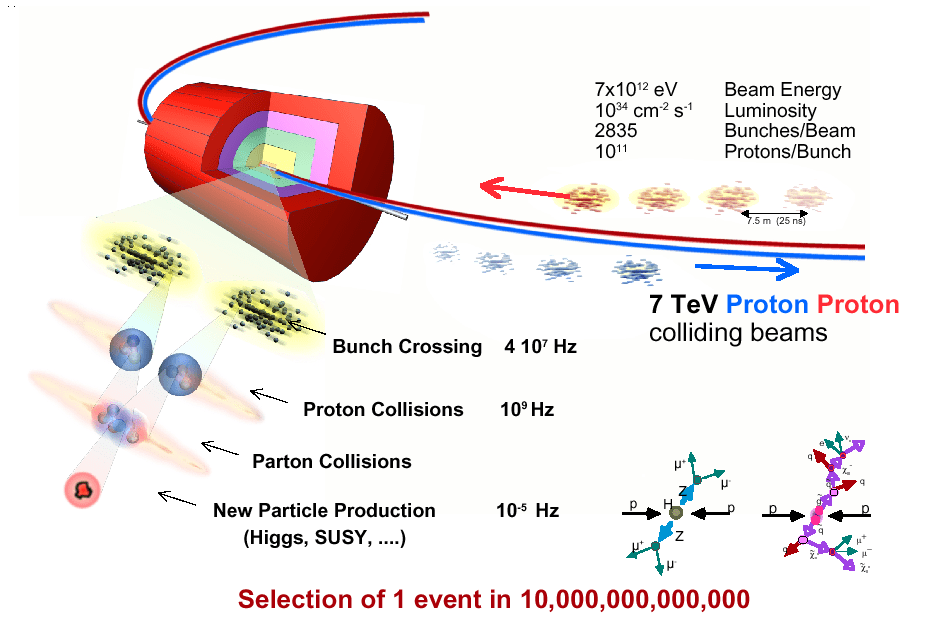
\includegraphics[scale=0.2]{Imag/sketch_collisions.png}
%    \caption{Representac\'on de las colisiones en el Gran Colisionador de Hadrones}
    \label{fig:my_label}
\end{figure}
    
\end{frame}


\begin{frame}{Modelo Dark-SUSY}

\begin{itemize}
    \item Producci\'on de fotones oscuros por medio del portal del Higgs 
    \item En este modelo el Higgs decae a particulas supersimetricas (neutralinos $n_{1}$)
    \item subsequentemente cada neutralino decae a un neutralino oscuro ($n_{D}$) y un fot\'on oscuro ($\gamma_{D}$)
    \tiem Cada fot\'on oscuro decae a un par de muones de carga opuesta
\end{itemize}

\begin{figure}
    \centering
    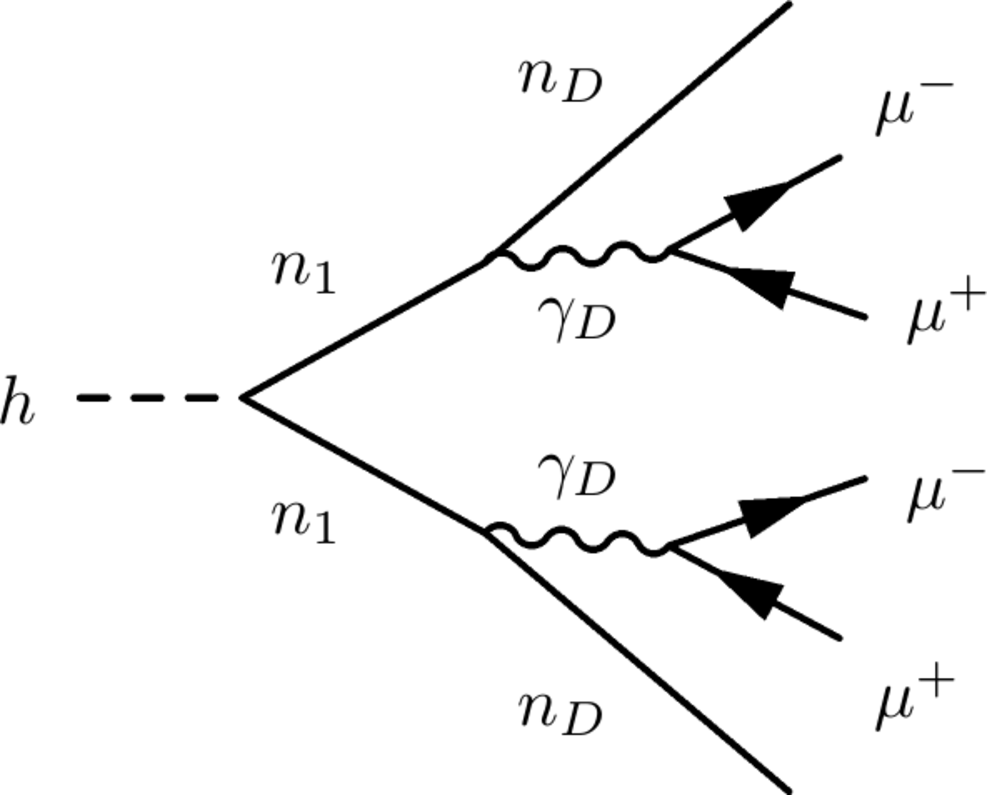
\includegraphics[scale=0.3]{Imag/figures_diagrams_h_to_2n1_to_2nD2gD_to_2nD4mu.pdf}
    \caption{Diagrama de Feynman del modelo Dark-SUSY}
    \label{fig:my_label}
\end{figure}

\end{frame}


\begin{frame}{Modelo Dark-SUSY}
    
    Las nuevas fuerzas en el escenario Dark-SUSY puede asociarse al modelo est\'andar por medio de un termino de mezcla (kinetic mixing) que en forma de lagrangia tiene la siguiente forma: 
    
    \begin{align*}
       \mathcal{L}_{KM} &= - \frac{\epsilon}{2} F^{Y}_{\mu \nu} F^{D_{\mu \nu}} 
    \end{align*} 

donde $F^{Y}_{\mu nu} = \partial_{\nu}A_{\nu}^{D} - \partial_{\nu}A_{\nu}^{D}$ es el campo de fuerzas en el sector oscuro. El rango tipico de $\epsilon$ es en el rango $10^{-8}$ - $10^{-2}$.
    
\end{frame}

\begin{frame}{Modelo Dark-SUSY: Decaimiento del foton oscuro a leptones}

\begin{itemize}
    \item Debido al factor de mezcla $\epislon$ el foton oscuro decae a leptones del modelo estandar con una anchura parcial dada por la siguiente expresion: 
    
    \begin{equation}
        \Gamma_{\gamma_{D}}\rightarrow \bar{l}l =\frac{1}{3}\alpha\epsilon^{2}m_{\gamma_{D}}\sqrt{1-\frac{4m_{l}^{2}}{m_{\gamma_{D}}^{2}}}\left(1+\frac{2m_{l}^{2}}{m_{\gamma_{D}}^{2}}\right)
    \end{equation}
\end{itemize}
    
Donde $m_{l}$ es la masa del lepton (e,$\mu$, or $\tau$)   
    
\end{frame}


\begin{frame}{Modelo Dark-SUSY: Tiempo de vida}

\begin{itemize}
    \item El tiempo de vida esta relacionado a la anchura de decaimiento con la siguiente expresión
\end{itemize}
    
    \begin{equation}
        \tau_{\gamma_{D}} = \frac{\hbar}{\Gamma_{\gamma_{D}}}
    \end{equation}
    
o también

\begin{equation}
    \tau(\epsilon, m_{\gamma_{D}}) = \frac{1}{\epsilon^{2}}\times f(m_{\gamma_{D}})
\end{equation}

Es decir el tiempo de vida es una función de la masa del fotón oscuro y el parámetro de mezcla $\epsilon$. 
    
\end{frame}


\begin{frame}{Modelo Dark-SUSY: Tiempo de vida}
    Es conveniente expresar el tiempo de vida como una distancia $c\tau_{\gamma_{D}}$, donde c es la velocidad de la luz. También es conveniente medir $c\tau_{\gamma_{D}}$ en milímetros para relacionar la sensitividad del modelo en el análisis de datos. 
    
    \begin{equation}
        c\tau_{\gamma_{D}}(\epsilon,m_{\gamma_{D}})[mm] = \frac{c[mm/s]\times \hbar[GeV.s]}{\epsilon^{2}} \times f(m_{\gamma_{D}}[GeV^{-1}]
    \end{equation}
    
    
\end{frame}

\begin{frame}{Propiedades del modelo}


    \begin{figure}[ht]
        \begin{minipage}[b]{0.45\linewidth}
            \centering
            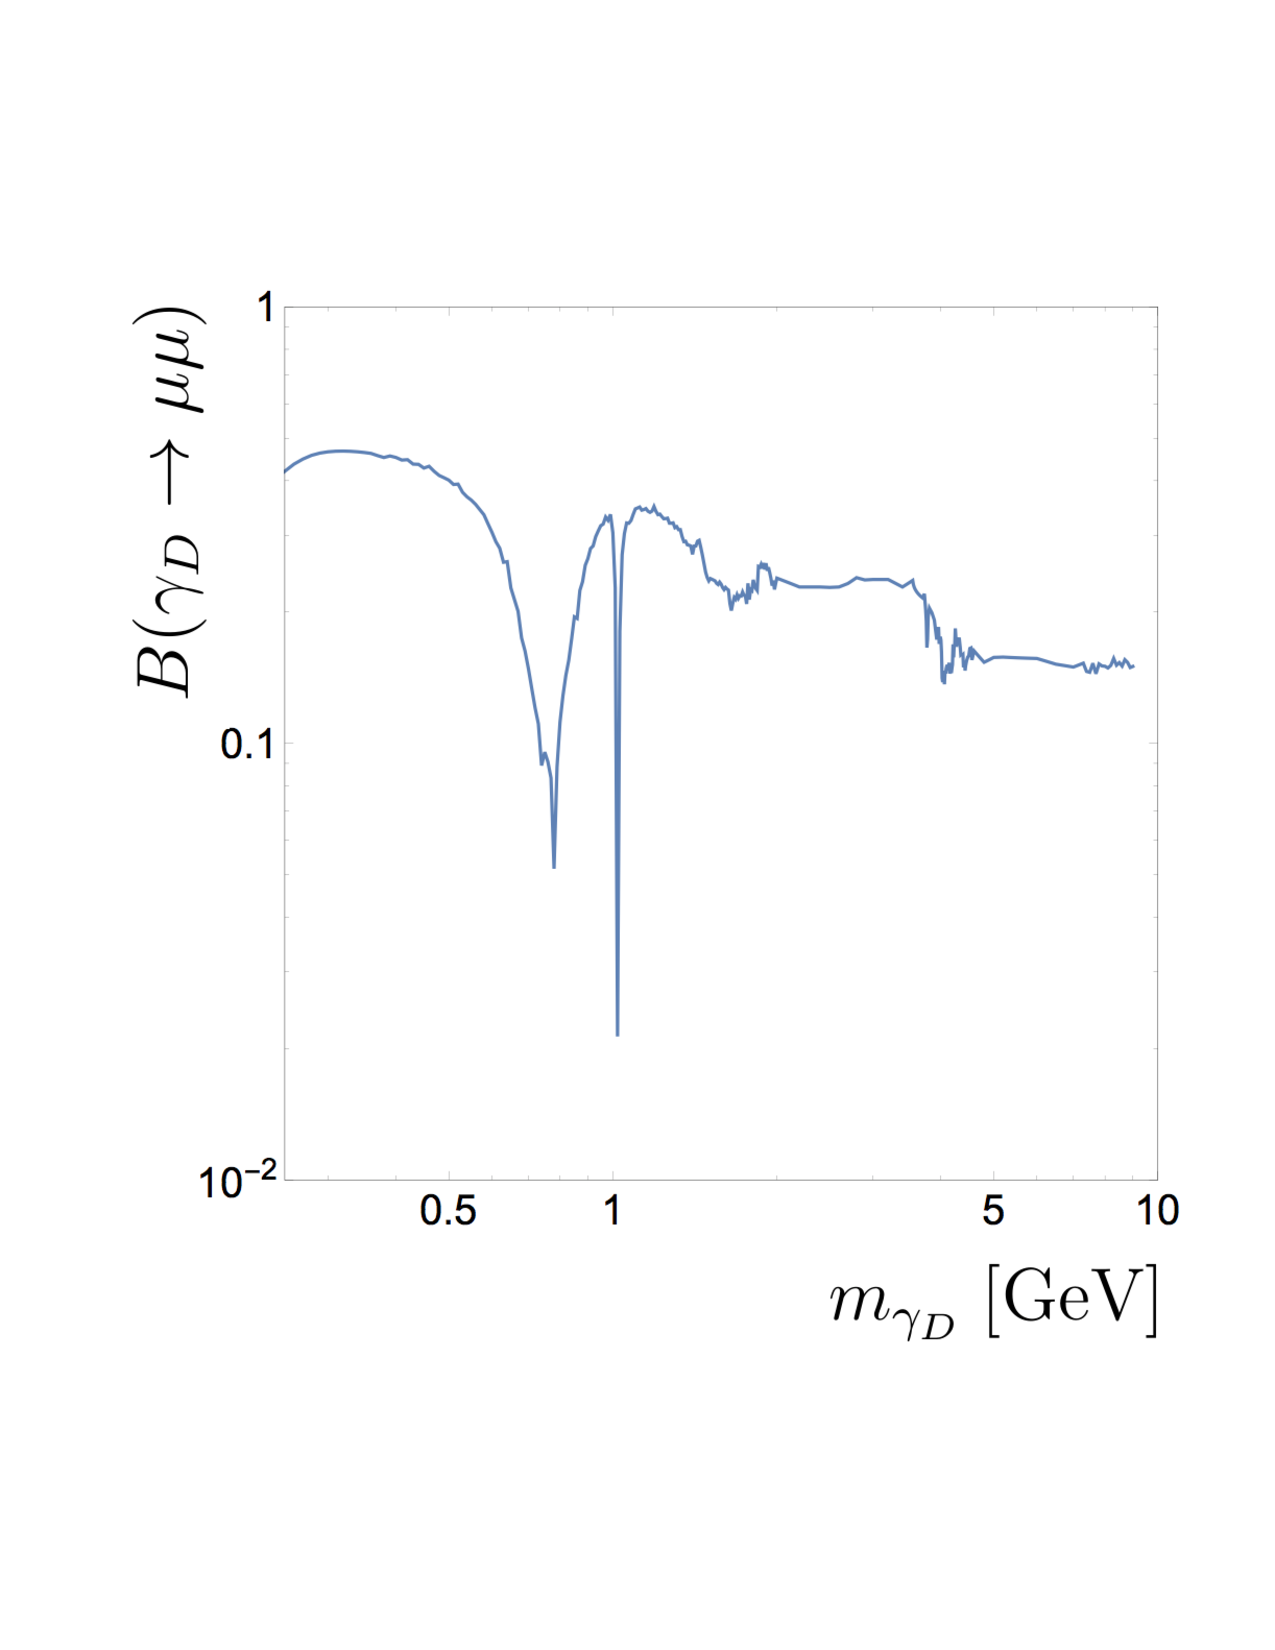
\includegraphics[width=\textwidth]{Imag/figures_intro_GammaD_BR_to_2mu_9GeVLog_updateTitles.pdf}
            \caption{Probabilidad de decaimiento del fotos oscuro a dos muones}
            \label{fig:a}
        \end{minipage}
        \hspace{0.5cm}
        \begin{minipage}[b]{0.45\linewidth}
            \centering
            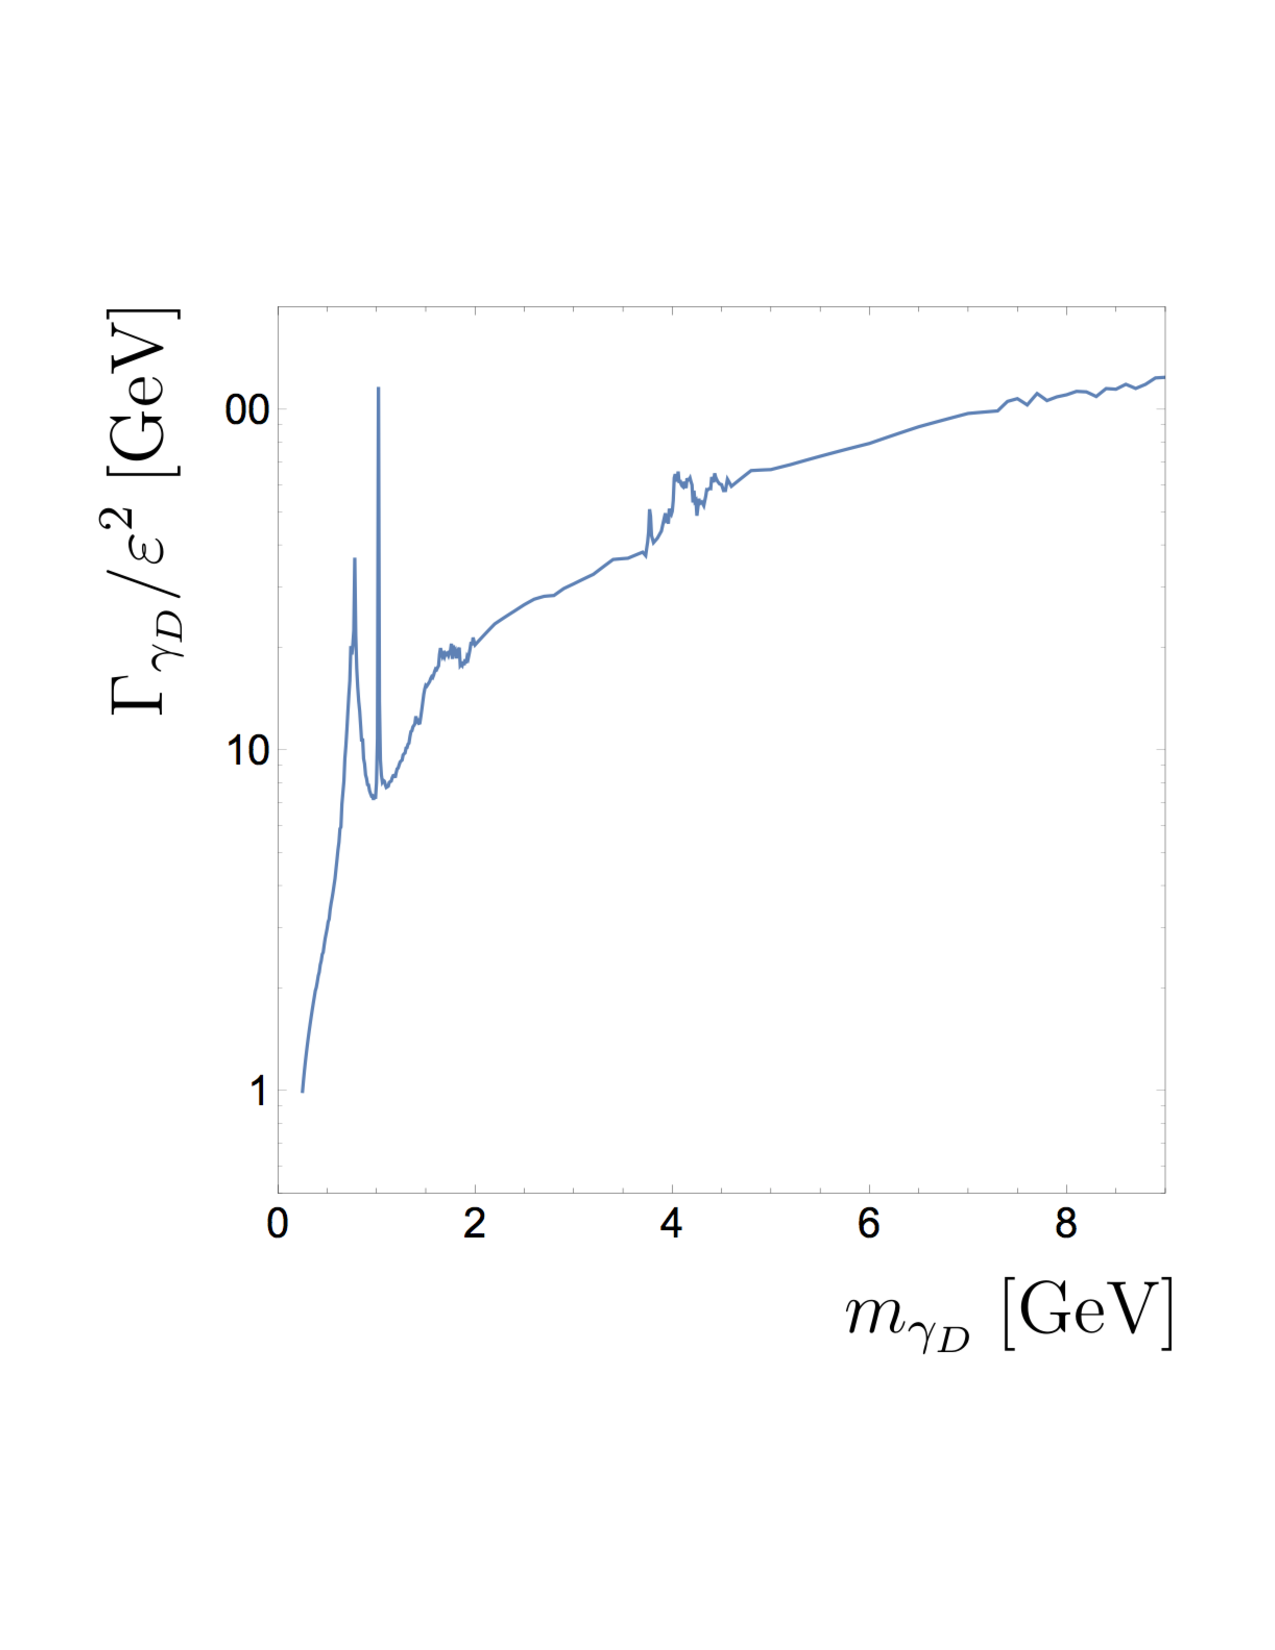
\includegraphics[width=\textwidth]{figures_intro_GammaD_Width_over_e2_GeV_upto9GeV_updatedTitles.pdf}
            \caption{Amplitud del decaimiento dividido por el coeficiente de mezcla cinetico}
            \label{fig:b}
        \end{minipage}
    \end{figure}

\end{frame}

